% To be compiled by XeLaTeX, preferably under TeX Live.
% LaTeX source for ``Yanqi Lake Lectures on Algebra'' Part III.
% Copyright 2019  李文威 (Wen-Wei Li).
% Permission is granted to copy, distribute and/or modify this
% document under the terms of the Creative Commons
% Attribution-NonCommercial 4.0 International (CC BY-NC 4.0)
% https://creativecommons.org/licenses/by-nc/4.0/

% To be included
\chapter{Primary decompositions}

We shall follow \cite[\S 3]{Eis95} and \cite[\S 8]{Mat80} closely.

\section{The support of a module}
Fix a ring $R$. For any $R$-module $M$ and $x \in M$, we define the \emph{annihilator} $\text{ann}_R(x) := \{ r \in R: rx=0 \}$; it is an ideal of $R$. Also define $\text{ann}_R(M) := \{r \in R: rM=0 \} = \bigcap_{x \in M} \text{ann}_R(x)$. \index{$\text{ann}_R(M), \text{ann}_R(x)$}

\begin{definition}\index{support}\index{SuppM@$\Supp(M)$}
	The \emph{support} of an $R$-module $M$ is
	\[ \Supp(M) := \left\{ \mathfrak{p} \in \Spec(R): M_{\mathfrak{p}} \neq 0 \right\}. \]
\end{definition}
Let us unwind the definition: $\mathfrak{p} \notin \Supp(M)$ means that every $x \in M$ maps to $0 \in M_{\mathfrak{p}}$, equivalently $\text{ann}_R(x) \not\subset \mathfrak{p}$. To test whether $\mathfrak{p} \notin \Supp(M)$, we only need to check the foregoing condition for $x$ ranging over a generating set of $M$.

\begin{proposition}
	If $M$ is finitely generated then $\Supp(M) = V(\mathrm{ann}_R(M))$; in particular it is Zariski-closed in $\Spec(R)$.
\end{proposition}
\begin{proof}
	Suppose $M = Rx_1 + \cdots + Rx_n$. Set $I_i := \text{ann}_R(x_i)$ and observe that $\bigcap_{i=1}^n I_i = \text{ann}_R(M)$. Then $\mathfrak{p} \in \Supp(M)$ if and only if $\mathfrak{p} \supset I_i$ for some $i$, that is, $\mathfrak{p} \in \bigcup_{i=1}^n V(I_i)$. To conclude, note that $V(I) \cup V(J) = V(IJ) = V(I \cap J)$ for any ideals $I, J \subset R$ (an easy exercise).
\end{proof}

Finite generation is needed in the result above. Consider the $\Z$-module $M := \bigoplus_{a \geq 1} \Z/p^a \Z$. Its support is $\{p\}$ but $\mathrm{ann}(M) = \{0\}$.

\begin{proposition}
	For an exact sequence $0 \to M' \to M \to M'' \to 0$ we have $\Supp(M) = \Supp(M') \cup \Supp(M'')$. For arbitrary direct sums we have $\Supp(\bigoplus_i M_i) = \bigcup_i \Supp(M_i)$.
\end{proposition}
\begin{proof}
	Again, we use the exactness of localization for the first assertion. For $\mathfrak{p} \in \Spec(R)$ we have an exact $0 \to M'_{\mathfrak{p}} \to M_{\mathfrak{p}} \to M''_{\mathfrak{p}} \to 0$, hence $M_{\mathfrak{p}} \neq 0$ if and only if $\mathfrak{p} \in \Supp(M') \cup \Supp(M'')$. The second assertion is obvious.
\end{proof}

From an $R$-module $M$, one can build a ``field of modules'' over $\Spec(R)$ by assigning to each $\mathfrak{p}$ the $R_{\mathfrak{p}}$-module $M_{\mathfrak{p}}$, and $\Supp(M)$ is precisely the subset of $M_{\mathfrak{p}}$ over which the field is non-vanishing. This is how the support arises in algebraic geometry. A more precise description will require the notion of quasi-coherent sheaves on schemes.

\begin{exercise}
	Let $M$, $N$ be finitely generated $R$-modules. Show that $\Supp(M \dotimes{R} N) = \Supp(M) \cap \Supp(N)$. Hint: since localization commutes with $\otimes$, it suffices to prove that $M \dotimes{R} N \neq \{0\}$ when $M, N$ are both nonzero finitely generated modules over a local ring $R$. Nakayama's Lemma implies that $M \dotimes{R} \Bbbk$ and $\Bbbk \dotimes{R} N$ are both nonzero where $\Bbbk$ is the residue field of $R$. Now
	\[ (M \dotimes{R} \Bbbk) \dotimes{\Bbbk} (\Bbbk \dotimes{R} N) \simeq M \dotimes{R} (\Bbbk \dotimes{\Bbbk} \Bbbk) \dotimes{R} N \simeq (M \dotimes{R} N) \dotimes{R} \Bbbk \]
	is nonzero.
\end{exercise}

\section{Associated primes}
Throughout this section, $R$ will be a Noetherian ring.

\begin{definition}\index{associated prime}\index{$\text{Ass}(M)$}
	A prime ideal $\mathfrak{p}$ is said to be an \emph{associated prime} of an $R$-module $M$ if $\text{ann}_R(x) = \mathfrak{p}$ for some $x \in M$; equivalently, $R/\mathfrak{p}$ embeds into $M$. Denote the set of associated primes of $M$ by $\text{Ass}(M)$.
\end{definition}

\begin{example}
	For the $\Z$-module $M := \Z/n\Z$ with $n \in \Z_{> 1}$, one easily checks that $\text{Ass}(M)$ is the set of prime factors of $n$.
\end{example}

\begin{lemma}\label{prop:Ass-maximal}
	Consider the set $\mathcal{S} := \{ \mathrm{ann}_R(x) : x \in M, \; x \neq 0 \}$ of ideals, partially ordered by inclusion. Every maximal element in $\mathcal{S}$ is prime.
\end{lemma}
\begin{proof}
	Let $\mathfrak{p} = \text{ann}_R(x)$ be a maximal element of $\mathcal{S}$ and suppose $ab \in \mathfrak{p}$. If $b \notin \mathfrak{p}$, then
	\[ bx \neq 0, \quad abx = 0, \quad R \neq \text{ann}_R(bx) \supset \text{ann}_R(x) = \mathfrak{p}. \]
	Hence $a \in \text{ann}_R(bx) = \mathfrak{p}$ by the maximality of $\mathfrak{p}$ in $\mathcal{S}$.
\end{proof}

\begin{definition}\index{zero divisor}
	Call $r \in R$ a \emph{zero divisor} on $M$ if $rx=0$ for some $x \in M \smallsetminus \{0\}$.
\end{definition}

\begin{theorem}\label{prop:Ass-properties}
	Let $M$ be an $R$-module.
	\begin{enumerate}[(i)]
		\item We have $M = \{0\}$ if and only if $\mathrm{Ass}(M) = \emptyset$.
		\item The union of all $\mathfrak{p} \in \mathrm{Ass}(M)$ equals the set of zero divisors on $M$.
		\item For any multiplicative subset $S \subset R$, we have
			\[ \mathrm{Ass}(M[S^{-1}]) = \left\{ \mathfrak{p}[S^{-1}] : \mathfrak{p} \in \mathrm{Ass}(M), \; \mathfrak{p} \cap S = \emptyset \right\} . \]
		\item If $0 \to M' \to M \to M''$ is exact, then $\mathrm{Ass}(M') \subset \mathrm{Ass}(M) \subset \mathrm{Ass}(M') \cup \mathrm{Ass}(M'')$.
	\end{enumerate}
\end{theorem}
\begin{proof}
	\begin{asparaenum}[(i)]
	\item Clearly $\text{Ass}(\{0\}) = \emptyset$. If $M \neq 0$, the set $\mathcal{S}$ in Lemma \ref{prop:Ass-maximal} is then nonempty, hence contains a maximal element $\mathfrak{p}$ because $R$ is Noetherian; this yields $\mathfrak{p} \in \text{Ass}(M)$.
	
	\item Elements of any $\mathfrak{p} \in \text{Ass}(M)$ are all zero divisors by the very definition of associated primes. Conversely, if $r \in \text{ann}_R(x)$ for some $x \in M \smallsetminus \{0\}$, there must exist some maximal element $\mathfrak{p}$ of $\mathcal{S}$ with $\mathfrak{p} \supset \text{ann}_R(x)$ as $R$ is Noetherian; so $\mathfrak{p}$ is the required associated prime containing $r$.
	
	\item If $\mathfrak{p} \in \Spec(R)$, $\mathfrak{p} \cap S = \emptyset$ and there is some $R/\mathfrak{p} \hookrightarrow M$, then
	\[ \{0\} \neq R[S^{-1}]/\mathfrak{p}[S^{-1}] \simeq (R/\mathfrak{p})[S^{-1}] \hookrightarrow M[S^{-1}] \]
	by the exactness of localizations, hence $\mathfrak{p}[S^{-1}] \in \text{Ass}(M[S^{-1}])$. Conversely, every element of $\text{Ass}(M[S^{-1}])$ has the form $\mathfrak{p}[S^{-1}]$ for some $\mathfrak{p} \in \Spec(R)$ disjoint from $S$. Also recall that $\mathfrak{p}$ equals the preimage of $\mathfrak{p}[S^{-1}]$ under $R \to R[S^{-1}]$. There exist $x \in M$ and $s \in S$ such that $\mathfrak{p}[S^{-1}] = \text{ann}_{R[S^{-1}]}(x/s) = \text{ann}_{R[S^{-1}]}(x)$. Ideals in a Noetherian ring being finitely generated, we infer that $\exists t \in S$ with $\mathfrak{p} \subset \text{ann}_R(tx)$. It remains to show $\mathfrak{p} = \text{ann}_R(tx)$. If $rtx=0$ for some $r \in R$, then $r$ maps into $r/1 \in \mathfrak{p}[S^{-1}] = \text{ann}_{R[S^{-1}]}(x)$; thus $r \in \mathfrak{p}$.

	\item It suffices to treat the second $\subset$. Suppose that $\mathfrak{p} \in \text{Ass}(M)$ and $R/\mathfrak{p} \simeq N$ for some submodule $N \subset M$. Identify $M'$ with $\Ker(M \to M'')$. If $M' \cap N = \{0\}$ then $R/\mathfrak{p} \simeq N \hookrightarrow M''$, so $\mathfrak{p} \in \text{Ass}(M'')$. If there exists $x \in M' \cap N \subset N$ with $x \neq 0$, then we have $\text{ann}_R(x) = \mathfrak{p}$ since $N \simeq R/\mathfrak{p}$ and $\mathfrak{p}$ is prime; in this case $\mathfrak{p} \in \text{Ass}(M')$.
	\end{asparaenum}
\end{proof}

We remark that $0 \to M' \to M \to M'' \to 0$ being exact does not imply $\text{Ass}(M) = \text{Ass}(M') \cup \text{Ass}(M'')$. To see this, consider $R=\Z$ and $0 \to \Z \xrightarrow{p} \Z \to \Z/p\Z \to 0$ for some prime number $p$.

\begin{exercise}
	Show that $\text{Ass}(M_1 \oplus M_2) = \text{Ass}(M_1) \cup \text{Ass}(M_2)$.
\end{exercise}

\begin{theorem}\label{prop:Supp-Ass}
	For every $R$-module $M$ we have $\Supp(M) = \bigcup_{\mathfrak{p} \in \mathrm{Ass}(M)} V(\mathfrak{p})$, in particular $\mathrm{Ass}(M) \subset \Supp(M)$.	Furthermore, every minimal element of $\Supp(M)$ with respect to inclusion is actually a minimal element of $\mathrm{Ass}(M)$.
\end{theorem}
\begin{proof}
	For any prime $\mathfrak{q}$ we have $M_{\mathfrak{q}} \neq 0 \iff \text{Ass}(M_{\mathfrak{q}}) \neq \emptyset$, and the latter condition holds precisely when there exists $\mathfrak{p} \in \text{Ass}(M)$ with $\mathfrak{p} \cap (R \smallsetminus \mathfrak{q}) = \emptyset$, i.e. $\mathfrak{q} \supset \mathfrak{p}$. This proves the first assertion. The second assertion is a direct consequence.
\end{proof}

Observe that if $\mathfrak{p} \in \Supp(M)$, then $\mathfrak{q} \supset \mathfrak{p} \implies \mathfrak{q} \in \Supp(M)$: the reason is that
\begin{gather}\label{eqn:localization-in-stages}
	M_{\mathfrak{p}} = (M_{\mathfrak{q}})_{\mathfrak{p}R_{\mathfrak{q}}}
\end{gather}
thus the occurrence of non-minimal elements in $\Supp(M)$ is unsurprising. In contrast, the non-minimal elements in $\text{Ass}(M)$ are somehow mysterious. These non-minimal associated primes are called \emph{embedded primes}. \index{embedded prime}

\begin{exercise}
	Prove the formula \eqref{eqn:localization-in-stages} of ``localization in stages''.
\end{exercise}

Hereafter we impose finite generation on $M$. This implies $M$ is Noetherian.
\begin{theorem}
	Let $M$ be a finitely generated $R$-module. There exists a chain $M = M_n \supset M_{n-1} \supset \cdots \supset M_0 = \{0\}$ of submodules such that for every $0 < i \leq n$, the subquotient $M_i/M_{i-1}$ is isomorphic to $R/\mathfrak{p}_i$ for some prime ideal $\mathfrak{p}_i$.
	
	Furthermore we have $\mathrm{Ass}(M) \subset \{\mathfrak{p}_1, \ldots, \mathfrak{p}_n \}$; in particular $\mathrm{Ass}(M)$ is a finite set.
\end{theorem}
\begin{proof}
	Assume $M \supsetneq M_0 := \{0\}$. There exists $\mathfrak{p}_1 \in \text{Ass}(M)$ together with a submodule $M_1 \subset M$ isomorphic to $R/\mathfrak{p}_1$. Furthermore $\text{Ass}(M_1) = \text{Ass}(R/\mathfrak{p}_1) = \{ \mathfrak{p}_1\}$ as easily seen. Hence the Theorem \ref{prop:Ass-properties} entails $\text{Ass}(M) \subset \{\mathfrak{p}_1\} \cup \text{Ass}(M/M_1)$.

	If $M_1 = M$ we are done. Otherwise we start over with $M/M_1$, finding $M_1 \subset M_2 \subset M$ with $M_2/M_1 \simeq R/\mathfrak{p}_2$ where $\mathfrak{p}_2 \in \text{Ass}_R(M/M_1)$, and so forth. This procedure terminates in finite steps since $M$ is Noetherian.
\end{proof}

\section{Primary and coprimary modules}
The classical framework of primary decompositions concerns ideals, but it is advantageous to allow modules here. As before, the ring $R$ is Noetherian.

\begin{definition}\index{coprimary module}\index{primary module}
	An $R$-module $M$ is called \emph{coprimary} if $\text{Ass}(M)$ is a singleton. A submodule $N \subsetneq M$ is called a $\mathfrak{p}$-\emph{primary} submodule if $M/N$ is coprimary with associated prime $\mathfrak{p} \in \Spec(R)$.
\end{definition}

\begin{proposition}\label{prop:coprimary-locnil}
	The following are equivalent for a nonzero $R$-module $M$.
	\begin{enumerate}[(i)]
		\item $M$ is coprimary;
		\item for every zero divisor $r \in R$ for $M$ and every $x \in M$, there exists $n \geq 1$ such that $r^n x = 0$.
	\end{enumerate}
\end{proposition}
The condition (ii) is usually called the local-nilpotency of $r$ on $M$. When $M = R/I$ for some ideal $I$, it translates into: all zero divisors of the ring $R/I$ are nilpotent.
\begin{proof}
	(i) $\implies$ (ii): Suppose $\text{Ass}(M) = \{ \mathfrak{p}\}$ and $x \in M \smallsetminus \{0\}$. From $\emptyset \neq \text{Ass}(Rx) \subset \text{Ass}(M)$ we infer that $\text{Ass}(Rx) = \{\mathfrak{p}\}$, thus by Theorem \ref{prop:Supp-Ass} we see $V(\mathfrak{p}) = \Supp(Rx) = V(\text{ann}(Rx))$. Hence $\mathfrak{p} = \sqrt{\text{ann}(Rx)}$. This implies (ii) by the definition of $\sqrt{\hspace{5pt}}$.
	
	(ii) $\implies$ (i): It is routine to check that
	\[ \mathfrak{p} := \left\{ r \in R: \forall x \in M \; \exists n \geq 1, \; r^n x = 0 \right\} \]
	is an ideal of $R$. For every $\mathfrak{q} \in \text{Ass}(M)$ there exists $x \in M$ with $\text{ann}_R(x) = \mathfrak{q}$. Every $r \in \mathfrak{p}$ has some power falling in $\mathfrak{q}$, thus $\mathfrak{p} \subset \mathfrak{q}$. Conversely, (ii) and Theorem \ref{prop:Ass-properties} imply $\mathfrak{q} = \text{ann}_R(x) \subset \mathfrak{p}$. From $\mathfrak{q}=\mathfrak{p}$ we conclude $M$ is coprimary with the unique associated prime $\mathfrak{p}$.
\end{proof}

\begin{exercise}[Classical definition of primary ideals]\label{ex:primary-ideal}
	Let $I$ be a proper ideal of $R$. Show that $R/I$ is coprimary if and only if the following holds:
	\[ \forall a,b \in R, \; (ab \in I) \wedge (a \notin I) \implies \exists n \geq 1, \; b^n \in I. \]
	In this case we also say $I$ is a \emph{primary ideal} of $R$. Show that $\{\sqrt{I}\} = \text{Ass}(R/I)$ if $I$ is a primary ideal. Hint: apply Proposition \ref{prop:coprimary-locnil}.
\end{exercise}

\begin{exercise}\label{ex:maximal-primary}
	Let $\mathfrak{m}$ be a maximal ideal of $R$. Show that every ideal $I \subsetneq R$ containing some power of $\mathfrak{m}$ is primary, and $\text{Ass}(R/I) = \{\mathfrak{m}\}$. Hint: show that $\mathfrak{m}$ is the only prime ideal containing $I = \text{ann}_R(R/I)$.
\end{exercise}

\begin{lemma}\label{prop:intersection-primary}
	Let $\mathfrak{p} \in \Spec(R)$ and $N_1, N_2 \subset M$ are $\mathfrak{p}$-primary submodules. Then $N_1 \cap N_2$ is a $\mathfrak{p}$-primary submodule of $M$.
\end{lemma}
\begin{proof}
	We have $M/N_1 \cap N_2 \hookrightarrow M/N_1 \oplus M/N_2$. Since $N_1 \cap N_2 \neq M$, we have
	\[ \emptyset \neq \text{Ass}(M/N_1 \cap N_2) \subset \text{Ass}(M/N_1) \cup \text{Ass}(M/N_2) = \{\mathfrak{p}\} \]
	by Theorem \ref{prop:Ass-properties}.
\end{proof}

\section{Primary decomposition: the main theorem}
We still assume $R$ Noetherian and fix a finitely generated $R$-module $M$.

\begin{theorem}[Lasker--Noether]\label{prop:primary-decomp}\index{primary decomposition}
	Let $N \subsetneq M$ be an $R$-submodule. Then we can express $N$ as
	\[ N = M_1 \cap \cdots \cap M_n, \]
	for some $n \geq 1$ and primary $R$-submodules $M_i$, say with $\mathrm{Ass}(M/M_i) = \{\mathfrak{p}_i\}$ for $i = 1, \ldots, n$. Such a decomposition is called a \emph{primary decomposition} of $N$. We say it is \emph{irredundant} if none of the $M_i$ can be dropped, and \emph{minimal} if there is no such decomposition with fewer terms.
	\begin{enumerate}[(i)]
		\item We have $\mathrm{Ass}(M/N) \subset \{ \mathfrak{p}_1, \ldots, \mathfrak{p}_n \}$, equality holds when the decomposition is irredundant.
		\item If the decomposition is minimal, then for every $\mathfrak{p} \in \mathrm{Ass}(M/N)$ there exists a unique $1 \leq i \leq n$ with $\mathfrak{p} = \mathfrak{p}_i$; consequently $n = |\mathrm{Ass}(M/N)|$.
		\item Consider a primary decomposition of $N$. Let $S \subset R$ be any multiplicative subset, and assume without loss of generality that $\mathfrak{p}_1, \ldots, \mathfrak{p}_m$ are the primes among $\{\mathfrak{p}_1, \ldots, \mathfrak{p}_n \}$ which are disjoint from $S$, then $m \geq 1 \iff N[S^{-1}] \subsetneq M[S^{-1}]$ and
		\[ N[S^{-1}] = M_1[S^{-1}] \cap \cdots \cap M_m[S^{-1}] \]
		is a primary decomposition of the $R[S^{-1}]$-submodule $N[S^{-1}] \subsetneq M[S^{-1}]$; this decomposition of $N[S^{-1}]$ is minimal if the one for $N$ is.
	\end{enumerate}
\end{theorem}
Note that the ``irredundant'' condition in \cite[(8.D)]{Mat80} corresponds to minimality here. The rings whose ideals all have primary decompositions are called \emph{Laskerian rings}, thus part (i) of the Theorem says Noetherian implies Laskerian, but there exist non-Noetherian examples.

\begin{proof}
	Establish the existence of primary decompositions first. Replacing $M$ by $M/N$, we may assume $N = \{0\}$ from the outset. We claim that
	\begin{gather}\label{eqn:Lasker-Noether-aux}
		\forall \mathfrak{p} \in \text{Ass}(M), \; \exists Q(\mathfrak{p}) \subset M, \;
		\left\{ \begin{array}{l}
			Q(\mathfrak{p}) \text{ is } \mathfrak{p}\text{-primary}, \\
			\text{Ass}(Q(\mathfrak{p})) = \text{Ass}(M) \smallsetminus \{ \mathfrak{p} \}. 
		\end{array}\right.
	\end{gather}
	Granting this, $Q := \bigcap_{\mathfrak{p} \in \text{Ass}(M)} Q(\mathfrak{p})$ yields the required decomposition since $\text{Ass}(M)$ is finite and $\text{Ass}(Q) = \emptyset$.
	
	Establish \eqref{eqn:Lasker-Noether-aux} as follows. Put $\Psi := \{ \mathfrak{p} \}$. By Zorn's Lemma\index{Zorn's Lemma} we get a maximal element $Q(\mathfrak{q})$ from the set
	\[ \emptyset \neq \left\{  Q \subset M: \text{submodule}, \; \text{Ass}(Q) \subset \text{Ass}(M) \smallsetminus \Psi \right\} \]
	which is partially ordered by inclusion (details omitted, and you may also use the Noetherian property of $M$). Since
	\[ \text{Ass}(M) \subset \text{Ass}(M/Q(\mathfrak{p})) \cup \text{Ass}(Q(\mathfrak{p})), \]
	it suffices to show $\text{Ass}(M/Q(\mathfrak{p})) \subset \Psi$.  Let $\mathfrak{q} \in \text{Ass}(M/Q(\mathfrak{p}))$ so that there exists $M \supset Q' \supset Q(\mathfrak{p})$ with $Q'/Q(\mathfrak{p}) \simeq R/\mathfrak{q}$. Since $\text{Ass}(Q') \subset \text{Ass}(Q(\mathfrak{p})) \cup \{ \mathfrak{q} \}$, maximality forces $\mathfrak{q} \in \Psi$ (otherwise $\text{Ass}(Q') \subset \text{Ass}(M) \smallsetminus \Psi$), whence \eqref{eqn:Lasker-Noether-aux}. Now we turn to the properties (i) --- (iii).
	
	\begin{asparaenum}[(i)]
		\item The obvious embedding
		\[ M/N \hookrightarrow \bigoplus_{i=1}^n M/M_i \]
		together with Theorem \ref{prop:Ass-properties} yield $\text{Ass}(M/N) \subset \bigcup_{i=1}^n \text{Ass}(M/M_i) = \{ \mathfrak{p}_1, \ldots, \mathfrak{p}_n \}$.
		
		Now assume the given primary decomposition is irredundant, we have
			\begin{align*}
				\{0\} & \neq \frac{M_2 \cap \cdots \cap M_n}{N} = \frac{M_2 \cap \cdots \cap M_n}{M_1 \cap (M_2 \cap \cdots \cap M_n)} \\
				& \simeq \frac{M_1 + M_2 \cap \cdots \cap M_n}{M_1} \hookrightarrow M/M_1.
			\end{align*}
			Thus $\text{Ass}(M/N)$ contains $\text{Ass}((M_2 \cap \cdots \cap M_n)/N) = \{\mathfrak{p}_1\}$. Same for $\mathfrak{p}_2, \ldots, \mathfrak{p}_n$.
		\item Suppose $N = M_1 \cap \cdots \cap M_n$ is an irredundant primary decomposition, so that $\text{Ass}(M/N) = \{ \mathfrak{p}_1, \ldots, \mathfrak{p}_n \}$. If $\mathfrak{p}_i = \mathfrak{p}_j$ for some $1 \leq i \neq j \leq n$, Lemma \ref{prop:intersection-primary} will imply that $M_i \cap M_j$ is primary, leading to a shorter primary decomposition. This is impossible when the primary decomposition is minimal.
		\item Suppose $S \cap \mathfrak{p}_i = \emptyset$ (equivalently, $i \leq m$). By Theorem \ref{prop:Ass-properties} and the exactness of localization, $M_i[S^{-1}] \subset M[S^{-1}]$ will be $\mathfrak{p}_i[S^{-1}]$-primary. On the other hand $S \cap \mathfrak{p}_i \neq \emptyset$ implies $\text{Ass}((M/M_i)[S^{-1}]) = \emptyset$ by Theorem \ref{prop:Ass-properties}, thus $M[S^{-1}]/M_i[S^{-1}] = 0$. Since localization respects intersections, we obtain
		\[ N[S^{-1}] = \bigcap_{i=1}^m M_i[S^{-1}]. \]
		In particular $N[S^{-1}]$ is proper if and only if $m \geq 1$.
	
		It remains to show $\text{Ass}(M[S^{-1}]/N[S^{-1}])$ has $m$ elements if the original primary decomposition is minimal. Indeed, that set is just $\{ \mathfrak{p}[S^{-1}] : \mathfrak{p} \in \text{Ass}(M/N), \; \mathfrak{p} \cap S = \emptyset \}$ by Theorem \ref{prop:Ass-properties}, which equals $\{ \mathfrak{p}_1[S^{-1}], \ldots, \mathfrak{p}_m[S^{-1}] \}$ (distinct) by (ii).
	\end{asparaenum}
\end{proof}

A natural question arises: to what extent are minimal primary decompositions unique? For those $M_i$ whose associated primes are minimal in $\text{Ass}(M/N)$, the answer turns out to be positive.

\begin{corollary}\label{prop:p-primary-component}
	Let $N = M_1 \cap \cdots \cap M_n$ be a minimal primary decomposition of $N \subsetneq M$. Suppose that $M_1$ is $\mathfrak{p}$-primary where $\mathfrak{p} := \mathfrak{p}_1$ is a minimal element in $\mathrm{Ass}(M/N)$, then $M_1$ equals the preimage of $N_{\mathfrak{p}}$ under $M \to M_{\mathfrak{p}}$. Call it the $\mathfrak{p}$-\emph{primary component} of $N$.
\end{corollary}
\begin{proof}
	Recall the proof of Theorem \ref{prop:primary-decomp}, especially the part (iii); here we localize with respect to $S := R \smallsetminus \mathfrak{p}$. The minimality assumption entails
	\[ N_{\mathfrak{p}} = M_{1, \mathfrak{p}} \subset M_{\mathfrak{p}}. \]
	It remains to show that the preimage of $M_{1, \mathfrak{p}}$ under $M \to M_{\mathfrak{p}}$ equals $M_1$, in other words the injectivity of the natural map $M/M_1 \to (M/M_1)_{\mathfrak{p}} = M_{\mathfrak{p}}/M_{1, \mathfrak{p}}$. Indeed, $\bar{x} \in M/M_1$ maps to $0$ if and only if there exists $s \notin \mathfrak{p}$ with $s\bar{x}=0$, but Theorem \ref{prop:Ass-properties} implies that the zero divisors of $M/M_1$ must lie in $\mathfrak{p}$.
\end{proof}

It follows that the non-uniqueness of minimal primary decompositions can only arise from embedded primes in $\text{Ass}(M/N)$.

\section{Examples and remarks}
Primary decompositions are most often applied in the case $M = R$ and $N = I$ is a proper ideal. The goal is to express $I$ as an intersection of primary ideals. To begin with, let us take $R = \Z$. Observations:
\begin{itemize}
	\item The primary ideals of $R$ take the form $(p)^n$, where $n \geq 1$ and $p$ is a prime number or zero. This may be deduced from Exercise \ref{ex:primary-ideal} or directly from definitions.
	\item The irredundant primary decompositions of $\Z/n\Z$, for $n > 1$, corresponds to the factorization of $n$ into prime-powers. There are no embedded primes in this case; the irredundant primary decomposition is unique and automatically minimal.
\end{itemize}

\begin{exercise}
	Justify the foregoing assertions.
\end{exercise}

\begin{figure}[h]
	\centering 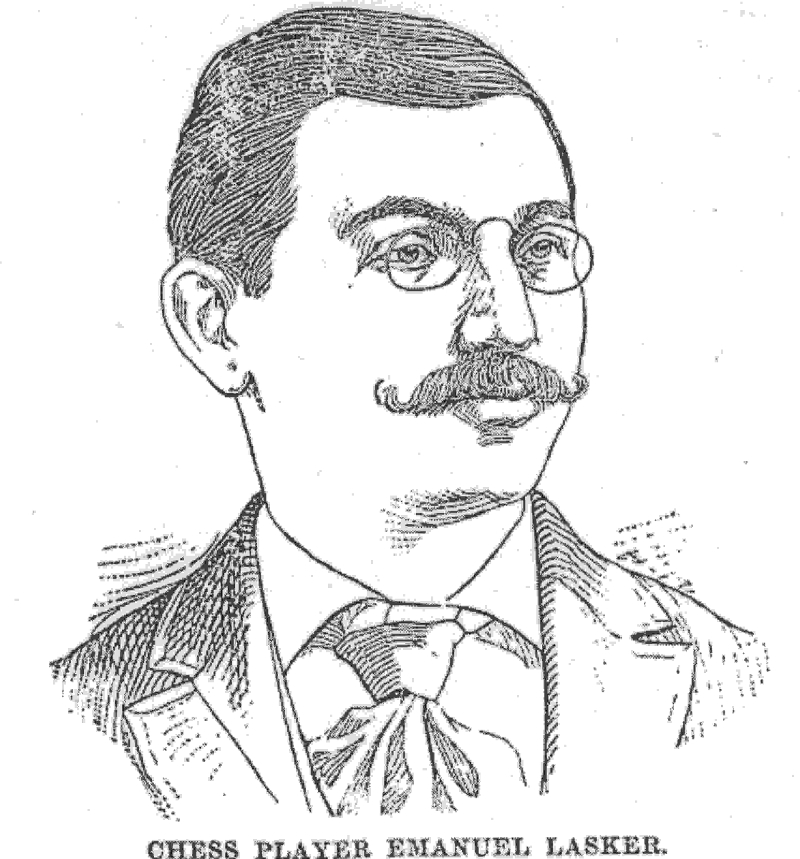
\includegraphics[height=170pt]{ELasker.jpg} \\ \vspace{1em}
	\begin{minipage}{0.7\textwidth}
		\small Emanuel Lasker (1868--1941) first obtained the primary decomposition for finitely generated $\Bbbk$-algebras and the algebras of convergent power series in 1905. His method involves techniques from \emph{elimination theory}. His result is then generalized and rewritten by Emmy Noether in 1921, in which the ascending chain condition plays a pivotal role. Lasker is best known for being the World Chess Champion from 1894 to 1921. (Picture taken from \href{https://commons.wikimedia.org/w/index.php?curid=5676713}{Wikimedia Commons})
	\end{minipage}
\end{figure}

Therefore one can regard primary decompositions as a generalization of factorization of integers, now performed on the level of ideals. The most important case is $R = \Bbbk[X_1, \ldots, X_n]$ (fix some field $\Bbbk$), as it is naturally connected to classical problems in algebraic geometry. Let us consider a simple yet non-trivial example from \cite[\S 3]{Eis95}.

\begin{example}
	Take $R=\Bbbk[X,Y]$ and $I = (X^2, XY)$. The reader is invited to check that
	\[ I = (X) \cap (X^2, XY, Y^2) = (X) \cap (X^2, Y). \]
	Claim: this gives two minimal primary decompositions of $I$. The ideal $(X)$ is prime, hence primary. In fact, $(X^2, XY, Y^2) = (X,Y)^2$ and $(X^2, Y)$ are both primary ideals associated to the maximal ideal $(X, Y)$. This follows either by direct arguments or by Exercise \ref{ex:maximal-primary}, noting that $(X,Y)^2 = (X^2, XY, Y^2)$ is contained in $(X^2, Y)$. The embedded prime $(X,Y)$ is seen to be responsible non-uniqueness of primary decompositions.
	
	To see the geometry behind, recall that $V(\mathfrak{a}) \cup V(\mathfrak{b}) = V(\mathfrak{a}\mathfrak{b}) = V(\mathfrak{a} \cap \mathfrak{b})$ for any ideals $\mathfrak{a}, \mathfrak{b}$, thus expressing $I$ as an intersection means breaking the corresponding geometric object into a union of simpler pieces. Also recall that for an ideal $I \subset \Bbbk[X,Y]$, the points in $\bigcap_{f \in I} \{f=0\}$ are in bijection with the maximal ideals lying over $I$, at least for $\Bbbk$ algebraically closed (Nullstellensatz). Thus we may interpret these primary decompositions as equalities among ``geometric objects'' embedded in $\Bbbk^2$:
	\[ \left\{ X^2=0, XY=0 \right\} = \begin{cases} \left\{ X = 0 \right\} \cup \left\{X^2=XY=Y^2=0 \right\} \\ \left\{ X = 0 \right\} \cup \left\{ X^2=Y=0 \right\}. \end{cases} \]
	\begin{enumerate}
		\item The geometric object defined by $X=0$ inside $\Bbbk^2$ is certainly the $Y$-axis: the regular functions living on this space form the $\Bbbk$-algebra $\Bbbk[X,Y]/(X) = \Bbbk[Y]$.
		\item The geometric object defined by $X^2=XY=Y^2=0$ looks ``physically'' like the origin $(0,0)$, but the $\Bbbk$-algebra of ``regular functions'' (in an extended sense) living on it equals $\Bbbk[X,Y]/(X^2,XY,Y^2)$: by restricting a polynomial function $f(X,Y)$ to this ``thickened point'', we see not only $f(0,0)$ but also $\frac{\partial f}{\partial x}(0,0)$ and $\frac{\partial f}{\partial y}(0,0)$. In other words, we shall view $X^2=XY=Y^2=0$ as the first-order infinitesimal neighborhood of $(0,0) \in \Bbbk^2$.
		\item In a similar vein, $X^2=Y=0$ physically defines $(0,0)$, but by restricting $f$ to that thickened point, we retrieve $f(0,0)$ as well as $\frac{\partial f}{\partial x}(0,0)$. Therefore we obtain the first-order infinitesimal neighborhood of $0$ inside the $X$-axis.
	\end{enumerate}

	Both decomposition says that we obtain the $Y$-axis together with first-order infinitesimal information at the origin $(0,0)$. This is also a nice illustration of the use of nilpotent elements in scheme theory.
\end{example}

\begin{example}[Symbolic powers]
	Let $\mathfrak{p}$ be a prime ideal in a Noetherian ring $R$ and fix $n \geq 1$. Observe that $\mathfrak{p}$ is the unique minimal element in $\Supp(R/\mathfrak{p}^n) = V(\mathfrak{p}^n)$. By Theorem \ref{prop:Supp-Ass} $\mathfrak{p} \in \text{Ass}(R/\mathfrak{p}^n)$, so it makes sense to denote by $\mathfrak{p}^{(n)}$ the $\mathfrak{p}$-primary component (Corollary \ref{prop:p-primary-component}) of $\mathfrak{p}^n$, called the $n$-th \emph{symbolic power} of $\mathfrak{p}$. In general $\mathfrak{p}^{(n)} \supsetneq \mathfrak{p}^n$. For a nice geometric interpretation of symbolic powers due to Nagata and Zariski, we refer to \cite[\S 3.9]{Eis95}.
\end{example}

Getting primary decomposition of ideals in polynomial algebras is a non-trivial task. Thanks to the pioneers in computational commutative algebra, this can now achieved on your own computer, eg. by the open-source \href{http://www.sagemath.org}{SageMath} system.\index{SageMath}